%! Tex Root = edp.tex
\documentclass[../edp.tex]{subfiles}

\begin{document}

{\scshape \hfill 30 de Marzo, 2023}

\subsection{Función de Green para el semiespacio}

Como dijimos antes, definir la función de Green depende de que podamos resolver
el problema corrector. En esta subsección resolveremos tal problema para el
semiespacio
\begin{displaymath}
	\R^{n}_{+}
	\coloneqq
	\lbrace 
		(x', x_n) \in \R^{n-1}\times\R^n
		\colon
		x_n > 0
	\rbrace
	\quad
	n \ge 3.
\end{displaymath}
Concretamente, debemos resolver, para \(x\in\R^{n}_{+}\) el problema
\begin{displaymath}
\begin{cases}
\begin{aligned}
	\Delta \varphi^{x}(y) &= 0 &&, y\in \R^n_{+}\\
	\varphi^{x}(y) &= \Phi(y - x) &&, y \in \partial\R^{n}_{+}
\end{aligned}
\end{cases}.
\end{displaymath}

Lo natural viendo las condiciones de borde, sería querer que
\(\varphi^{x}(\cdot) = \Phi(\cdot - x)\), y de hecho, tenemos que 
\begin{displaymath}
	\Delta_{y} \Phi(y-x) = 0,
\end{displaymath}
siempre y cuando \(y\ne x \in \R^{n}_{+}\). El problema aquí es que nos falta un
punto y nuestra función debe estar definida sobre todo el semiespacio. Por otro
lado, la función \(\Phi\) no tiene más singularidades, así que
\begin{displaymath}
	\Delta_{y} \Phi(y - \tilde{x}) = 0
	,\quad \forall \tilde{x}\not\in\overline{\R^{n}_{+}}.
\end{displaymath}
\begin{wrapfigure}{r}{0.3\textwidth}
\hspace{2em}
\begin{tikzpicture}[scale=1.5]
	\draw[-] (-0.1,0) -- (2,0);
	\draw[->] (0, -1) -- (0,1);

	\coordinate (y) at (.25,0);
	\coordinate (x) at (30:1);
	\coordinate (x') at (-30:1);

	\draw[fill=black] (y) circle(1pt) node[below] {\(y\)};
	\draw[fill=black] (x) circle(1pt) node[above,right] {\(x\)};
	\draw[fill=black] (x') circle(1pt) node[below,right] {\(\tilde{x}\)};

	\draw[dashed] (y) -- (x);
	\draw[dashed] (y) -- (x');
\end{tikzpicture}
\end{wrapfigure}
Así, si podemos encontrar un \(\tilde x\) tal que se satisfagan las
condiciones de borde habremos resuelto el problema. Y en efecto, usando las
simetrías del semiespacio, se nota que si \(y\in\partial\R^{n}_{+}\) entonces
los puntos \(x = (x', x_n) \in \R^{n}_{+}\) y \(\tilde x = (x', -x_n)
\in\R^{n}_{-}\) están a la misma distancia y por lo tanto
\begin{displaymath}
	\varphi^{x}(y)
	=
	\Phi(y - x) 
	= 
	\Phi(y - \tilde{x}).
\end{displaymath}
Definimos entonces \(\varphi^{x}(y) = \Phi(y - \tilde{x})\), y por lo tanto la
fórmula de Green se lee
\begin{displaymath}\label{Green:semiplano}
	G(x,y) = \Phi(y-x) - \Phi(y-\tilde{x}).
	\tag{GS}
\end{displaymath}
Más aún, por la fórmula de representación, cualquier solución \(u\) del problema
\begin{displaymath}\label{poisson:semiespacio}
\begin{cases}
\begin{aligned}
	-\Delta u &= 0 &&, \text{ en } \R^n_{+}\\
	u &= g &&, \text{ en } \partial\R^{n}_{+}
\end{aligned}
\end{cases},
\tag{PS}
\end{displaymath}
se escribe como
\begin{align*}\label{representacion:semiespacio}
	u(x)
	=
	- \int_{\partial\R^{n}_{+}}
		g(y) \partial_{n(y)} G(x,y) \, dS(y)
	=
	\int_{\partial\R^{n}_{+}}
		g(y) \frac{2 x_n}{n \alpha(n) \abs{x-y}^{n}}\, dS(y).
	\tag{FPS}
\end{align*}
Esta fórmula es conocida como \textbf{fórmula de Poisson} para el semiespacio,
además, el \textbf{kernel de Poisson} se define como:
\begin{displaymath}\label{kernel de poisson:semiespacio}
	k(x,y) 
	\coloneqq
	\frac{2 x_n}{n \alpha(n)}
	\frac{1}{\abs{x-y}^{n}}
	,\quad y\in \partial\R^{n}_{+}, x\in \R^{n}_{+}.
	\tag{KPS}
\end{displaymath}

Vamos a comprobar que~\eqref{representacion:semiespacio}, en efecto, resuelve el
problema~\eqref{poisson:semiespacio}.

\begin{Teorema}
	Si \(g\in \CC(\R^{n-1}) \cap L^{\infty}(\R^{n-1})\) y \(u\) está dado
	por~\eqref{representacion:semiespacio}, entonces
	\begin{enumerate}
		\item \(u\in \C^{\infty}(\R^n_{+}) \cap L^{\infty}(\R^n_{+})\);
		\item \(\Delta u = 0\) en el semiespacio; y
		\item Si \(x_0 \in \partial\R^{n}_{+}\) entonces 
		\begin{displaymath}
			\lim_{\R^{n}_{+} \ni x\to x_0} u(x) = g(x_0).
		\end{displaymath}
	\end{enumerate}
\end{Teorema}
\begin{Demostracion}
	Sabemos que \(G(x,y)\) es tal que \(\Delta_{y} G(x,y) = 0\). Ahora, como
	\(G(x,y)\) es simétrica, se sigue que \(\Delta_{x} G(x,y) = 0\). Luego,
	\begin{align*}
		\Delta_{x} u(x)
		&=
		\Delta_{x}
		- \int_{\partial\R^{n}_{+}}
			g(y) \partial_{n(y)} G(x,y) \, dS(y)
		\\&=
		- \int_{\partial\R^{n}_{+}}
			g(y) 
			\Delta_{x} \partial_{n(y)} G(x,y) \, dS(y)
		\\&=
		- \int_{\partial\R^{n}_{+}}
			g(y) 
			\partial_{\n(y)} 
			\underbrace{\Delta_{x} G(x,y)}_{=0} 
			\, dS(y)
		= 0.
	\end{align*}
	Por lo tanto \(\Delta u = 0\) en el semiespacio y por lo tanto también es
	\(\CC^{\infty}\). Para ver que es integrable, basta ver que
	\(\partial_{\n(y)} G(x,y)\) es integrable. Vamos a ello.

	\begin{wrapfigure}{r}{0.3\textwidth}
	\hspace{2em}
	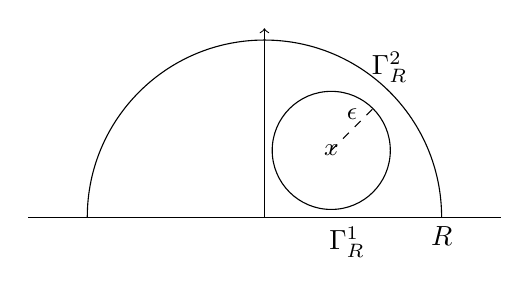
\begin{tikzpicture}[scale=1.5]
		\draw[-] (-2,0) -- (2,0);
		\draw[->] (0,0) -- (0,1.6);
		\draw (45:.8) circle(0.5) 
			node {\small\(x\)};
		\draw[dashed] (45:.8) -- (45:1.3) 
			node[midway, above] {\small\(\epsilon\)};
		\draw (1.5,0) arc(0:180:1.5) 
			node[below, at start] {\(R\)}
			node[near start, above] {\(\Gamma_{R}^{2}\)};
		\node[below] at (.7,0) {\(\Gamma_{R}^{1}\)};
	\end{tikzpicture}
	\end{wrapfigure}
	Sea \(x\in \R^{n}_{+}\). Tomemos \(R\gg 1\) tal que \(x\in B(0,R)\) y
	\(\epsilon \ll 1\) tal que \(B(x,\epsilon) \subset B(0,R)\cap \R^{n}_{+}\).
	Miremos la región \(\Theta_{R,\epsilon} \coloneqq B(0,R) \cap
	(\R^{n}_{+} \setminus B(x,\epsilon))\). Sabemos que
	\begin{displaymath}
		0 = \int_{\Theta_{R,\epsilon}} \Delta_{y} G(x,y) \, dS(y)
	\end{displaymath}
	Llamemos \(\Gamma_{R}^{2}\) a la superficie de la bola que está en el
	semiespacio y \(\Gamma_{R}^{1}\) a la que toca el borde del subespacio. 
	Por el Teorema de la divergencia, la expresión anterior se
	lee
	\begin{displaymath}
		0
		=
		\int_{\Gamma_{R}^{2}}
			\partial_{\n(y)} G(x,y) \, dS(y)
		+
		\int_{\Gamma_{R}^{1}}
			\partial_{\n(y)} G(x,y) \, dS(y)
		+ 
		\int_{\partial B(x,\epsilon)}
			\partial_{\n(y)} G(x,y) \, dS(y)
	\end{displaymath}
	Tomando \(R \to \infty\) y \(\epsilon \to 0\) notamos que
	\begin{displaymath}
	\begin{aligned}
		(1) &&
		\int_{\Gamma_{R}^{1}}
			\partial_{\n(y)} G(x,y) \, dS(y)
		&=
		\int_{\partial \R^{n}_{+}} k(x,y)\, dS(y)\\
		(2) &&
		\abs{\int_{\Gamma_{R}^{2}} \partial_{\n(y)} G(x,y) \, dS(y)}
		&\le
		C/R \to 0\\
		(3) &&
		\int_{\partial B(x,\epsilon)}
			\partial_{\n(y)} G(x,y) \, dS(y)
		&=
		\underbrace{
		\int_{\partial B(x,\epsilon)}
			\partial_{\n(y)} \Phi(y-x) \, dS(y)
		}_{\to -1}
		+
		\underbrace{
		\int_{\partial B(x,\epsilon)}
			\partial_{\n(y)} \Phi(y-\tilde{x}) \, dS(y)
		}_{\to 0}
	\end{aligned}
	\end{displaymath}
	Así que
	\begin{equation}\label{KPS integra 1}
		\int_{\partial \R^{n}_{+}} k(x,y)\, dS(y)\\
		= 1,
	\end{equation}
	y por lo tanto \(u\in L^{\infty}(\R^{n}_{+})\).

	Finalmente, probaremos el tercer punto. Sea \(x_0 \in \partial\R^{n}_{+}\) 
	y \(x\in\R^{n}_{+}\). Por~\eqref{KPS integra 1} 
	y~\eqref{representacion:semiespacio} tenemos que
	\begin{align*}
		g(x_0) - u(x)
		&=
		g(x_0) - \int_{\partial\R^{n}_{+}} g(y) k(x,y)\, dS(y)
		\\&=
		\int_{\partial\R^{n}_{+}} (g(x_0) - g(y)) k(x,y)\, dS(y).
	\end{align*}

	Sea \(\epsilon > 0\) y tomemos \(\delta > 0\) tal que 
	\begin{displaymath}
		\abs{x_0 - y} < \delta
		\implies
		\abs{g(x_0) - g(y)} < \epsilon
		\qquad y \in \partial\R^{n}_{+}.
	\end{displaymath}

	Sea \(x\in B(x_0, \delta/2) \cap \R^{n}_{+}\). Entonces
	\begin{align*}
		\abs{g(x_0) - u(x)}
		&=
		\abs{
		\int_{\partial\R^{n}_{+}} 
			(g(x_0) - g(y)) k(x,y)\, dS(y)
		}
		\\&\le
		\int_{\partial\R^{n}_{+}} 
			\abs{g(x_0) - g(y)} \abs{k(x,y)} \, dS(y)
		\\&=
		\underbrace{
		\int_{\partial\R^{n}_{+} \cap B(x_0, \delta)} 
			\abs{g(x_0) - g(y)} \abs{k(x,y)} \, dS(y)
		}_{I}
		\\&+
		\underbrace{
		\int_{\partial\R^{n}_{+}\setminus\overline{B(x_0, \delta)}} 
			\abs{g(x_0) - g(y)} \abs{k(x,y)} \, dS(y)
		}_{J}.
	\end{align*}
	
	Por la continuidad de \(g\) y~\eqref{KPS integra 1}, tenemos que 
	\(I \le \epsilon \xrightarrow{\epsilon\to0} 0\). Por otro lado, para estimar
	\(J\), notemos que
	\begin{displaymath}
		\begin{aligned}
			\abs{x - x_0} &\le \delta/2\\
			\abs{y - x_0} &> \delta
		\end{aligned}
		\implies
		\abs{y - x} \ge \frac{1}{2} \abs{y-x_0}.
	\end{displaymath}
	De esta forma,
	\begin{displaymath}
		J 
		\le
		2 \norm{g}_{L^{\infty}}
		\int_{\partial\R^{n}_{+}\setminus\overline{B(x_0,\delta)}}
			k(x,y) \, dS(y)
		\le
		\frac{2^{n+2}}{n\alpha(n)} 
		\norm{g}_{L^{\infty}} x_n
		\int_{\partial\R^{n}_{+}\setminus\overline{B(x_0,\delta)}}
			\abs{y-x_0}^{-n} \, dS(y),
	\end{displaymath}
	y por lo tanto \(J \to 0\) cuando \(x_n \to 0\). Es decir, cuando \(x \to
	x_0\), \(\abs{g(x_0) - u(x)} \to 0\).
\end{Demostracion}

\end{document}
